\begin{frame}{Audiobooks on Storytel: Active Fanbase}
\note{
Leveraging publicly available data on Storytel, I analyzed the number of reviews and average ratings of each book.

\begin{itemize}
    \item The scatterplot reveals engagement with the series on Storytel. The y-axis represents the number of reviews (log scale), while the x-axis shows the audiobook release dates.
    \item The series began with a high of 1104 reviews, dwindling to 395 by the end. This suggests that not all readers rate every book they listen to, but those who reached the end likely read earlier titles.
    \item The series' dedication is clear: a median of 511 reviews per book, never dropping below 333.
    \item Storytel's release strategy was methodical, launching a new audiobook chapter every Thursday over 16 months. This maintained listener engagement and promoted sustained subscriptions.
\end{itemize}
}
    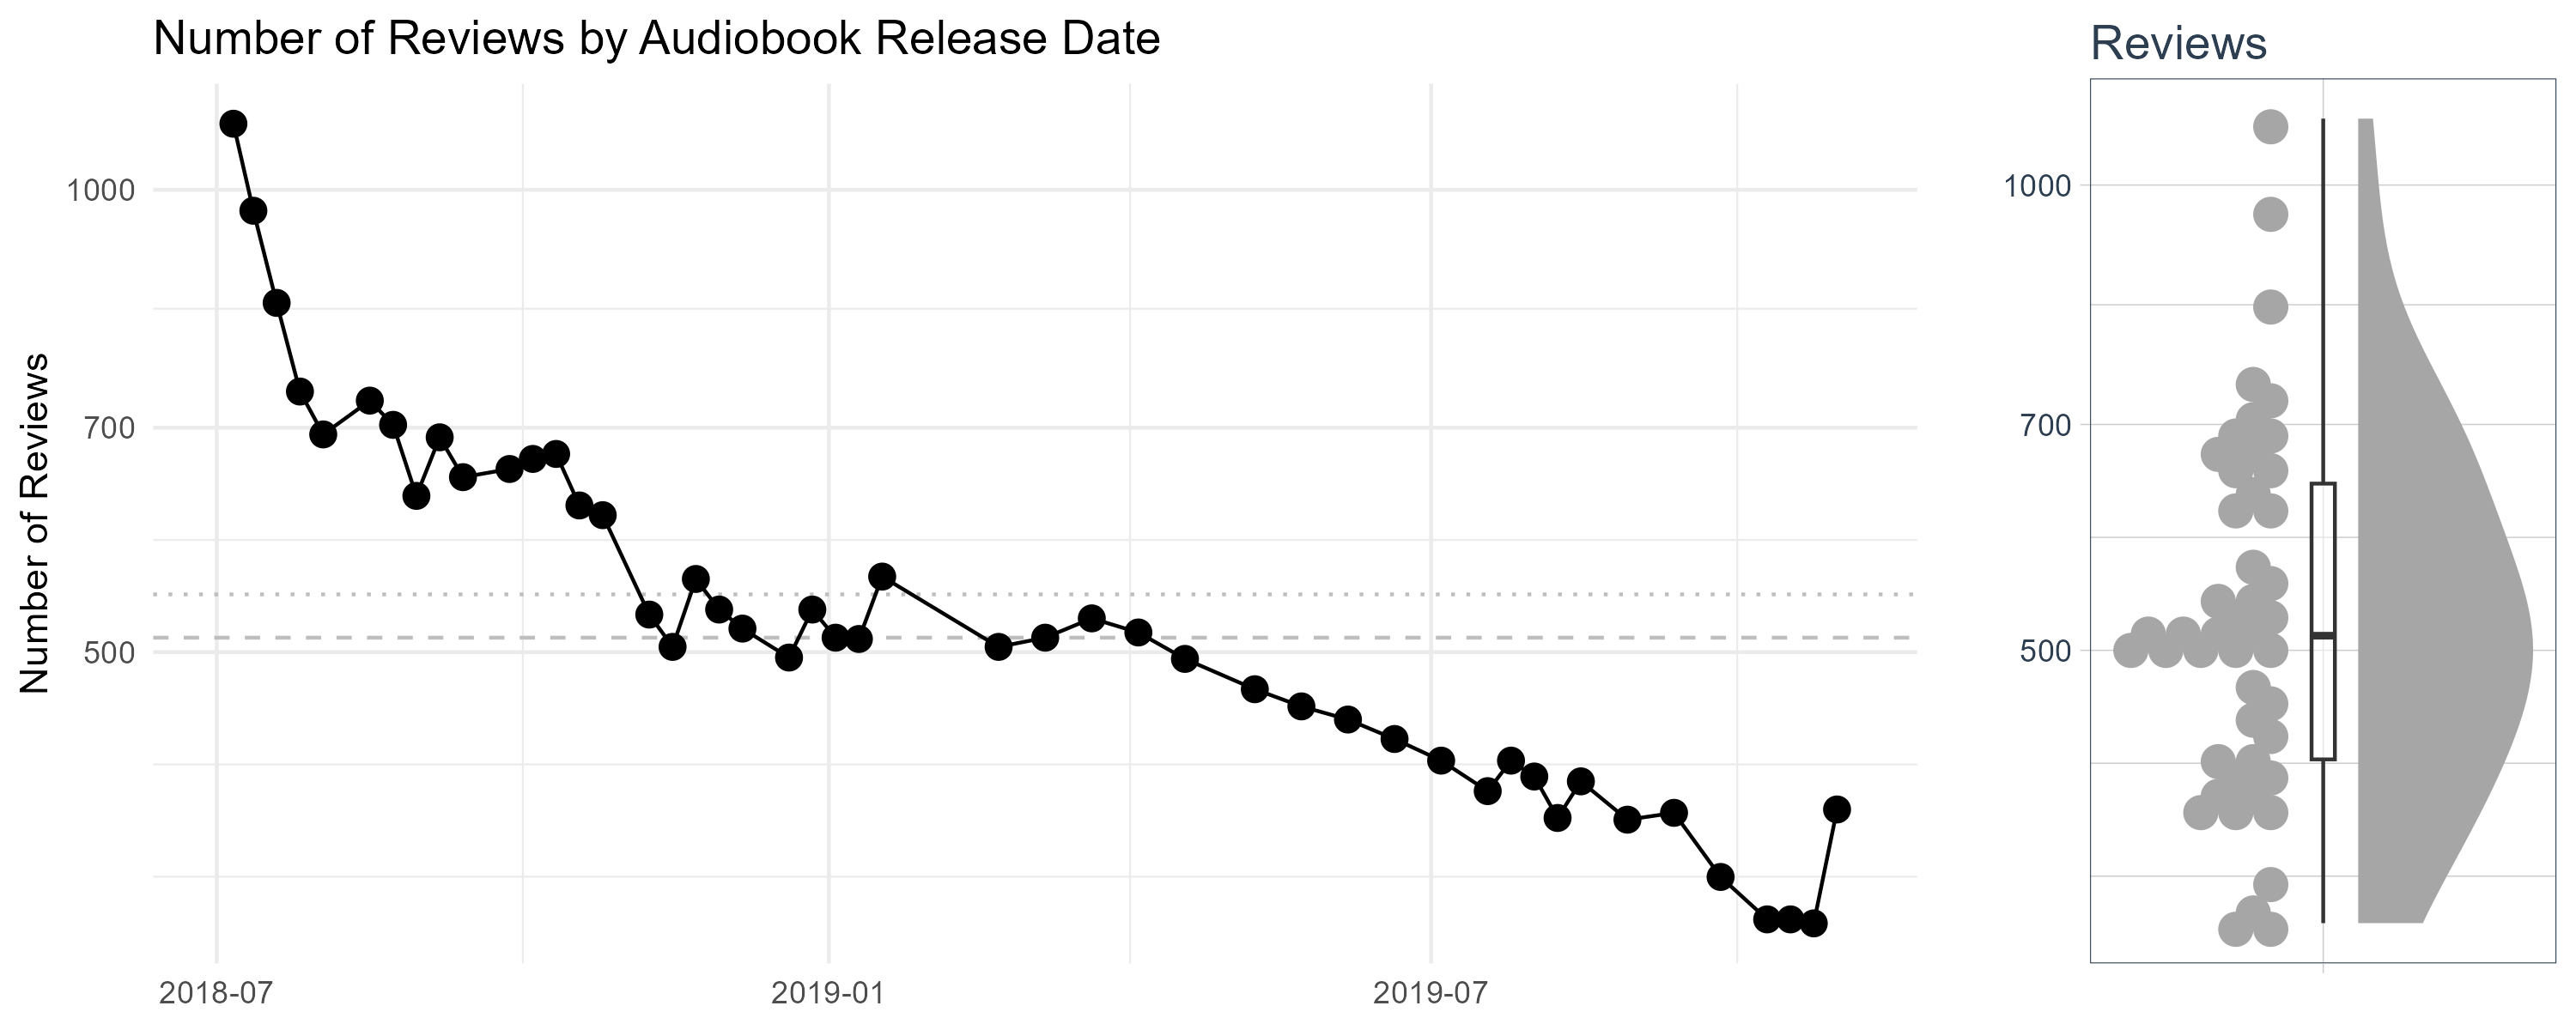
\includegraphics[width=\textwidth]{../R/figures/storytel_reviews}

    \begin{itemize}
    \item The series has a dedicated fanbase, with consistently high engagement.
    \item A solid median review count of 511, and minimum of 333.
    \item Releases on Thursdays, spaced 1--2 weeks apart, over 16-months.
    \end{itemize}

\end{frame}

\begin{frame}{Audiobooks on Storytel: High Ratings}
\note{
    \begin{itemize}
        \item Now, the y-axis showcases the series' mean ratings.

        \item Ratings stay consistently commendable, between 4.1 and 4.6 stars, with a median of 4.5 stars.

        \item It's key to note that Storytel combines e-book and audiobook ratings, which might blur distinctions between content and narration quality.

        \item A notable dip in ratings in the series' latter part matches Margit's admissions of writer's fatigue. This hints at the series' changing quality and readers' keen observations.
    \end{itemize}
}

    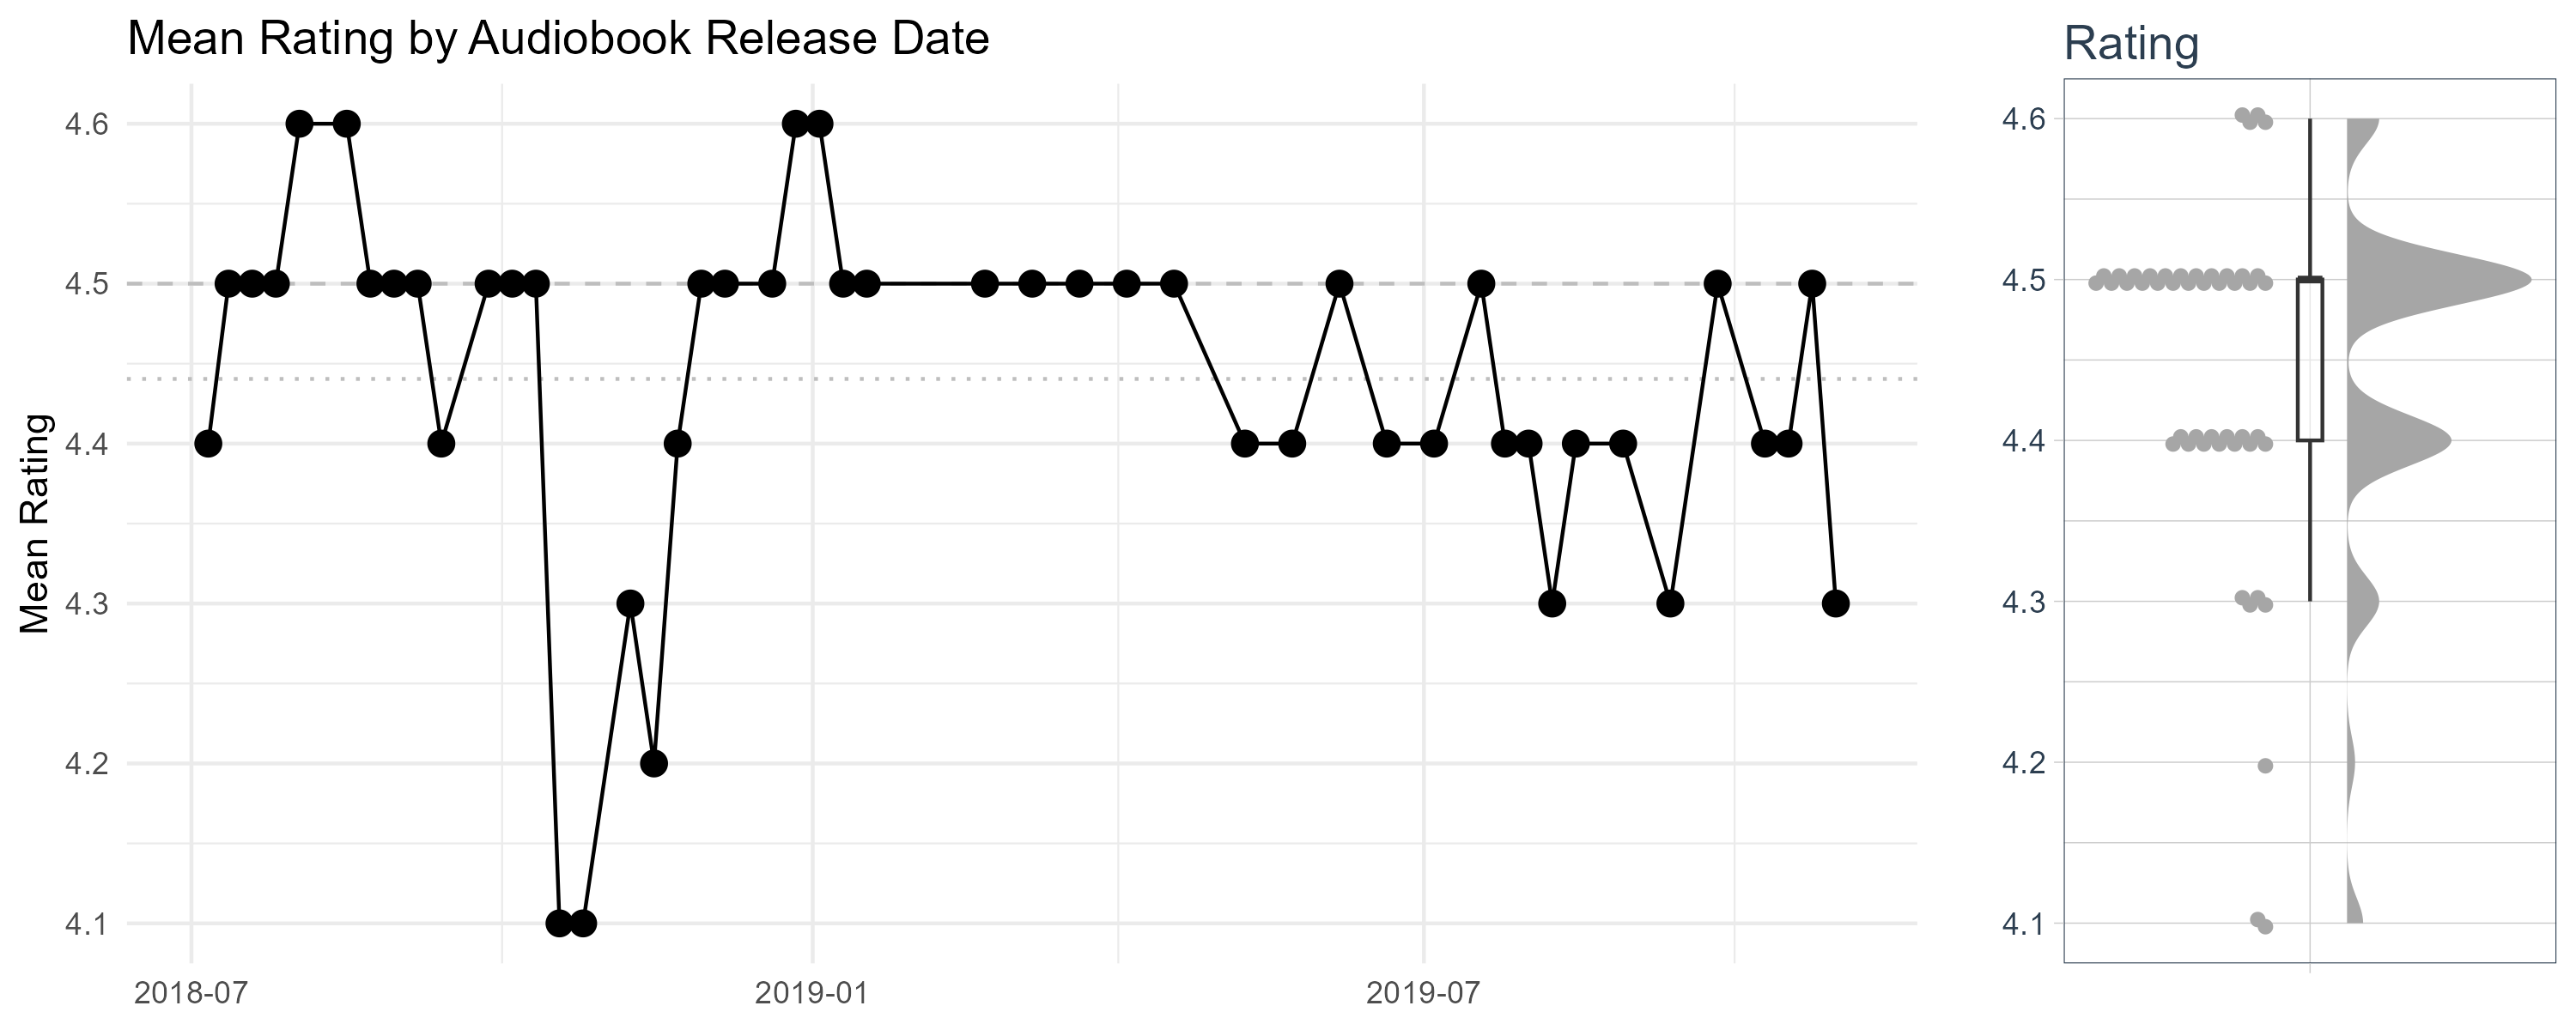
\includegraphics[width=\textwidth]{../R/figures/storytel_ratings}
    \begin{itemize}
    \item Overall high rating, an average 4.44 stars out of 5.
    \end{itemize}
\end{frame}

\begin{frame}{Audiobooks on Storytel: Our Narrators}
\note{
Shift your focus now to the narrators, who rendered 18,000 minutes (about 13 days) of medieval romantic fantasy.

The y-axis shows total narration hours per book.

\begin{itemize}
    \item Although the written book length decreased, audiobook durations increased.
    This could suggest narrators might have slowed down their reading pace.

    \item Rumor has it the first narrator left after a third of the series due to its intense and controversial themes.

    \item The second narrator tried to voice each character uniquely. This radio-play style, however, saw a dip in ratings.
    Though book content primarily influences ratings, changes in narration styles might also play a part.

    \item Ratings rebounded with the third narrator's traditional style. She narrated almost half the series.

    \item Kudos to the narrators for their distinct styles and dedication.
\end{itemize}
}
    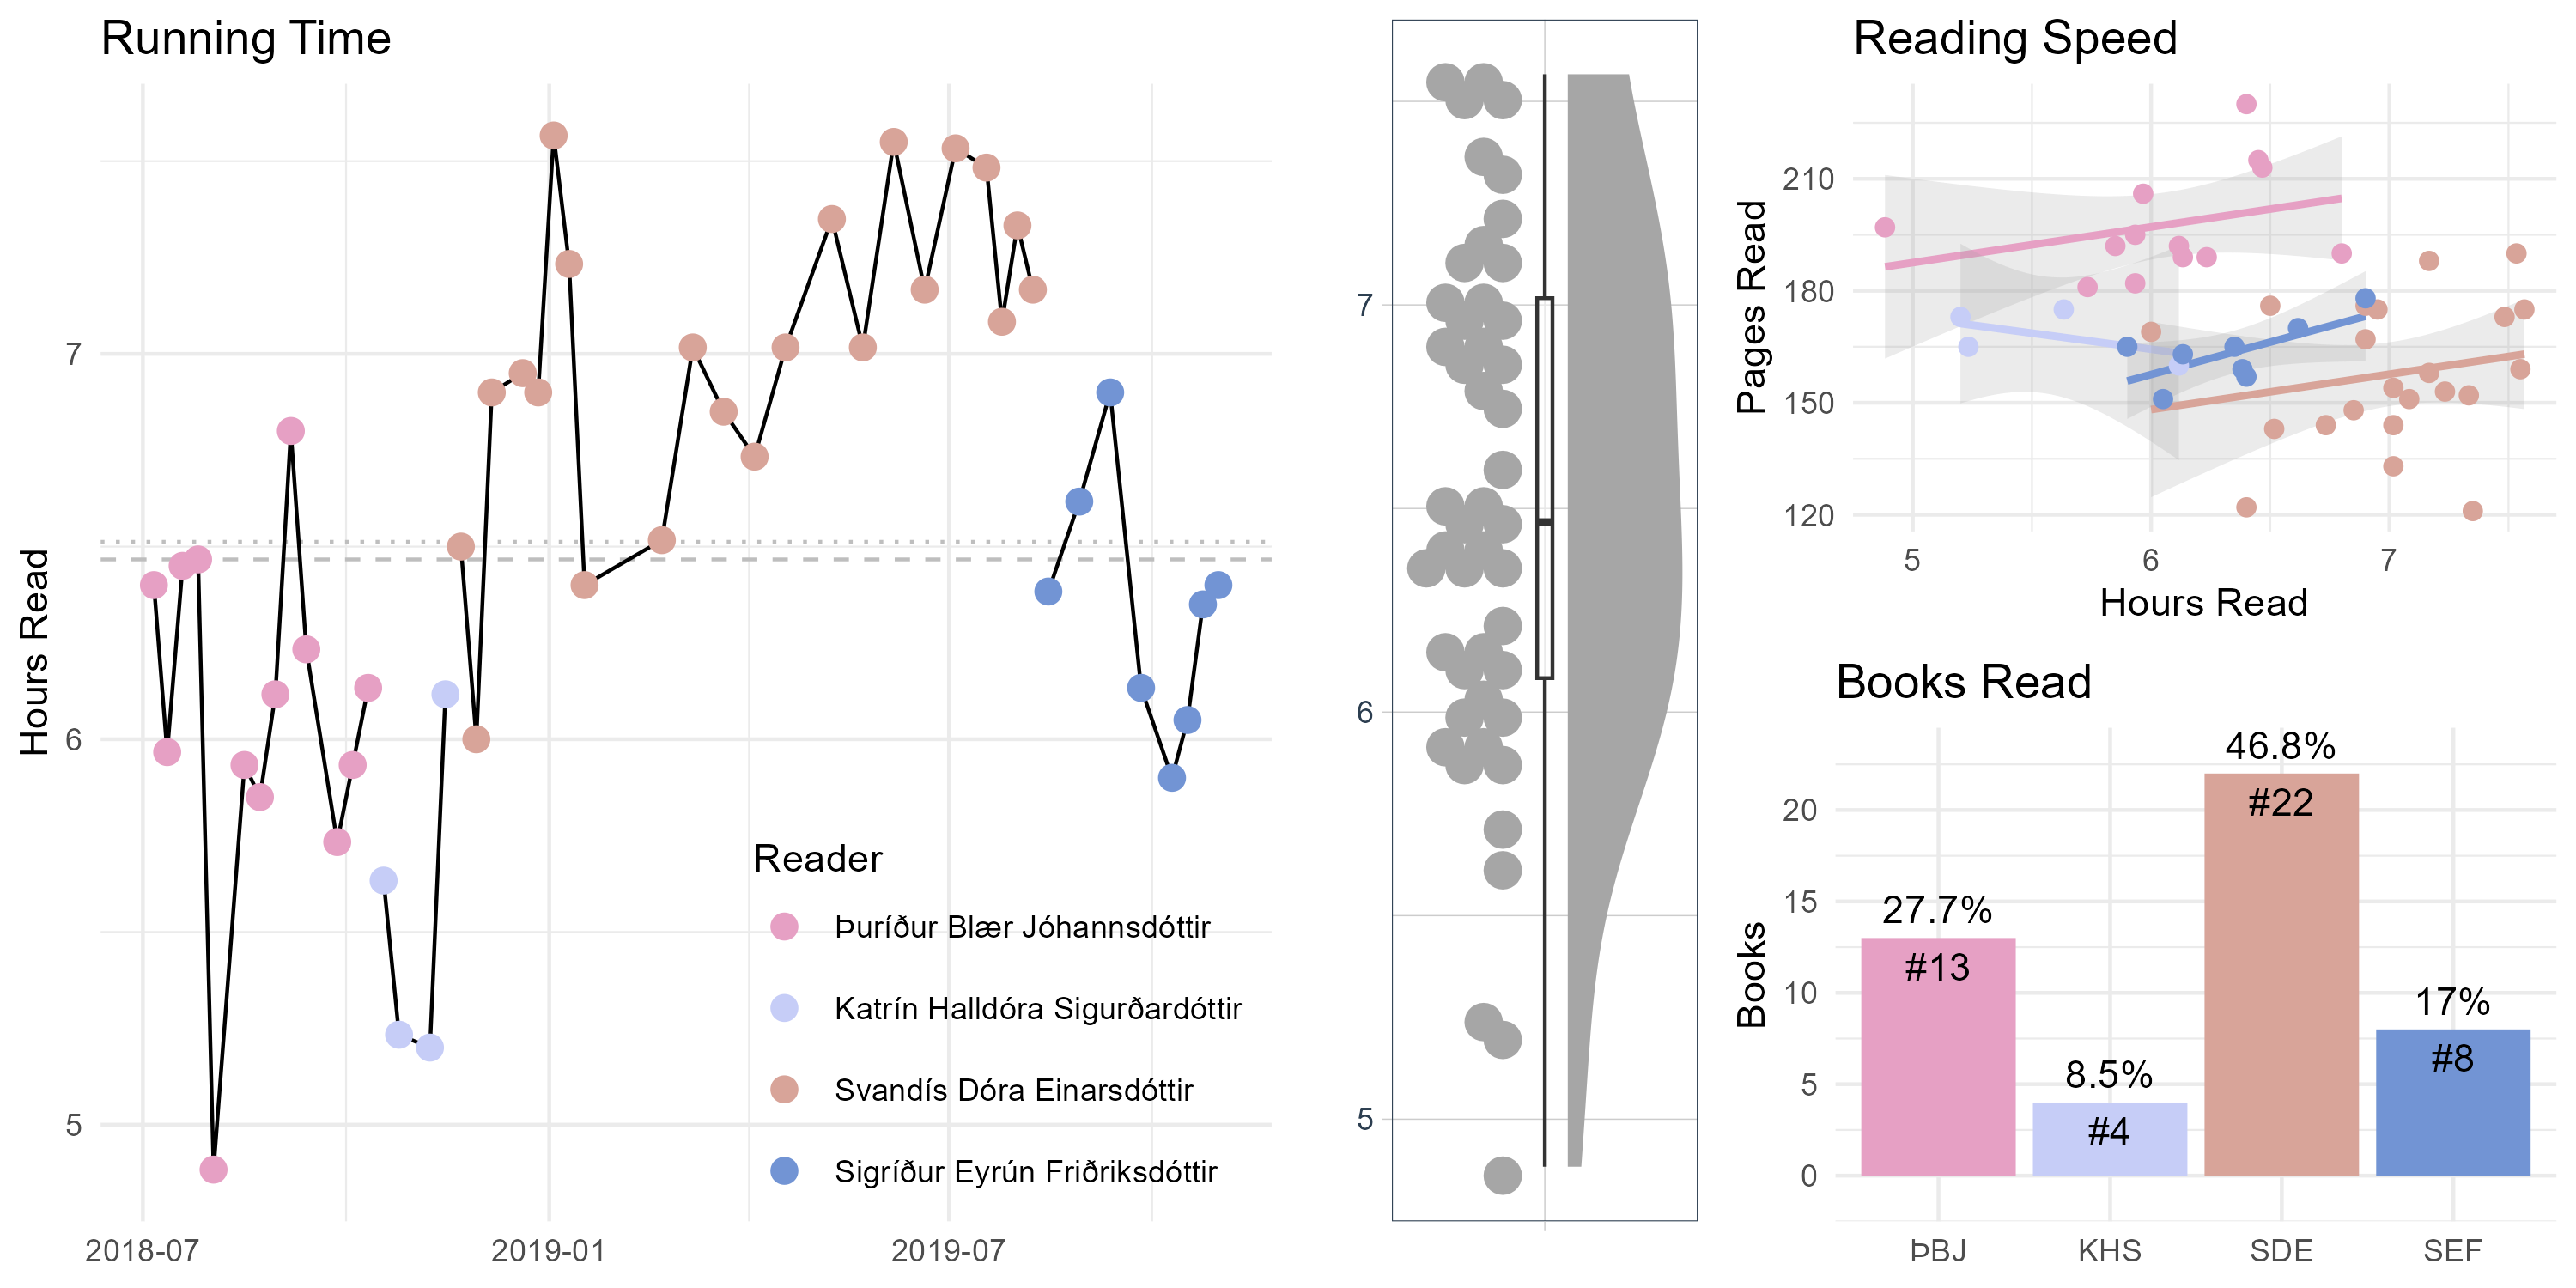
\includegraphics[width=\textwidth]{../R/figures/storytel_readers}
    \vspace{-18pt}
    \begin{itemize}
    \item Over 18K min of romantic medieval fantasy -- 12.8 days of cont. listening
    \item Four distinct voices with varied styles \& perseverance with Margit's prose
    \end{itemize}

\end{frame}
